\documentclass[a4paper]{article}

\usepackage[english]{babel}
\usepackage[utf8x]{inputenc}
\usepackage{amsmath}
\usepackage{amssymb}
\usepackage{amsthm}
\usepackage{graphicx}
\usepackage{tikz}
\usetikzlibrary{arrows,automata}
\usepackage[colorinlistoftodos]{todonotes}
\usepackage[margin=0.75in]{geometry}
\usepackage{enumerate}

\title{Discrete Math Assignment 6}
\author{Rachel Hwang}

\begin{document}
\maketitle

\begin{enumerate}

\item \emph{Prove that if $d_i,\dots, d_n$ is the degree sequence of a simple graph then the following two sequences also have this property:}
\begin{enumerate}[(a)]
\item $d_1,d_2+1,d_3, d_4, d_5, d_6, d_7+1, d_8,3, 1 (n = 8)$; \\
\\
Let the graph of the original degree sequence be $G = (V,E)$. We may create a new graph $G' = (V',E')$. We first add all $v \in V$ to $V'$ (assume $v_i \in V$ has degree $d_i$). We then also add two vertices $v_9$ and $v_{10}$. We can then add all edges in $E$ to $E'$ as well as edges $(v_9, v_{10})$, $(v_2, v_9)$, and $(v_7, v_9)$ to $E'$. It's clear that $v_9$ has degree 3 $v_{10}$ has degree 1, and $d_2$ has degree $d_2+1$ and $d_7$ has degree $d_7+1$. Since we have only added edges which use newly added vertices, we cannot have added an edge that was already in $E$. Since we have added no edges from any vertex to itself, we have added no loops. Since it has no loops and no multiple edges between the same two vertices, $G'$ is a simple graph. \\

\item $n-1-d_1,n-1-d_2,\dots n-1-d_n$.  \\
\\
Let the graph of the original degree sequence be $G = (V,E)$ and the set of all possible unique undirected edges $\{(u,v), u,v \in V\}$ be called $S$. We may create a new graph $G' = (V',E')$ where $V = V'$. $E' = \{(u,v) \in S | (u,v) \notin E\}$. Conceptually, this is like creating a complement graph for $G$. Since $n-1$ is the maximum possible degree for any vertex (which connects it to every other vertex in the graph), this means that each $v_i \in V'$ has degree $n-1-d_i$. By construction, $G'$ has no multiple edges, and no loops, so $G'$ is a simple graph. \\ \\
\end{enumerate}


\item \emph{Let $a,b \geq 2$ be integers. Consider the graph $G = (V,E)$ where $V = \{0,1,\dots, a-1\}$ and $E = \{(x,x+b\;mod\;a)|x \in V\}$. Prove that $G$ has exactly $gcd(a,b)$ connected components.} \\
\\
By Bezout's Theorem, we know that if $gcd(a, b) = d$, then there are some $x$ and $y$ such that $xa+yb = d$. So,
\begin{align*}
xa+yb &=d \\
yb &= d\; mod\; a \\
n + yb &= (d+n)\; mod\; a
\end{align*}
If we consider the $n$ above to represent the vertex that we are trying to find a connection for, this tells us that for any vertex number $n$, $n$ is connected to the vertex $n+d$. Likewise, $n+d$ is connected to $n+d+d$, and so on. However, because Bezout's Theorem also tells us that the $gcd(a, b)=d$ is the mimimum value for which there is a solution to $xa+yb =d$. This also tells us that $n$ will never be connected to a vertex $n+e$ where $e < d$. That is, for all number vertices greater than $n$ and less than $n+d$, $n$ cannot be connected to them. \\
\\
So, if we begin from $n = 0$, we have a sequence of connected vertices $0, 0+d,0+d+d, \dots$. If $d \neq 1$, because $0$ is not connected to $1$, that connected sequence is \emph{not} connected to the next sequence starting at 1, which is $1,1+d,1+d+d,\dots$. There is one such sequence for every number from $0$ to $d-1$, none of which connect to each other. Therefore, the number of connected components is $d = gcd(a,b)$. \\



\item \emph{How many $(s, t)$ paths of length five does the graph in Figure 1 contain?} \\
\\
There are 12 paths from $s$ to $t$. \\
\\
First, because we want paths of exactly length 5, we can disregard the vertical edges perpendicular to a straight line between $s$ and $t$. Since taking one of those edges does not advance towards $t$ and no other edges advance more than one step towards $t$, including one of these vertical edges would result in a path of length 6. \\
\\
Of the remaining edges, we can count the number of paths to each vertex $v$ as the sum of all the paths that lead to each point that connect to $v$ from some starting point. So, $paths(u,v) = \Sigma_w paths(w, v)$ where there is a path from $u$ to $w$. Using this method, the figure below labels each vertex with the number of paths to it from $s$. Clearly, we can observe that the number of patha from $s$ to $t$ is 12.\\

 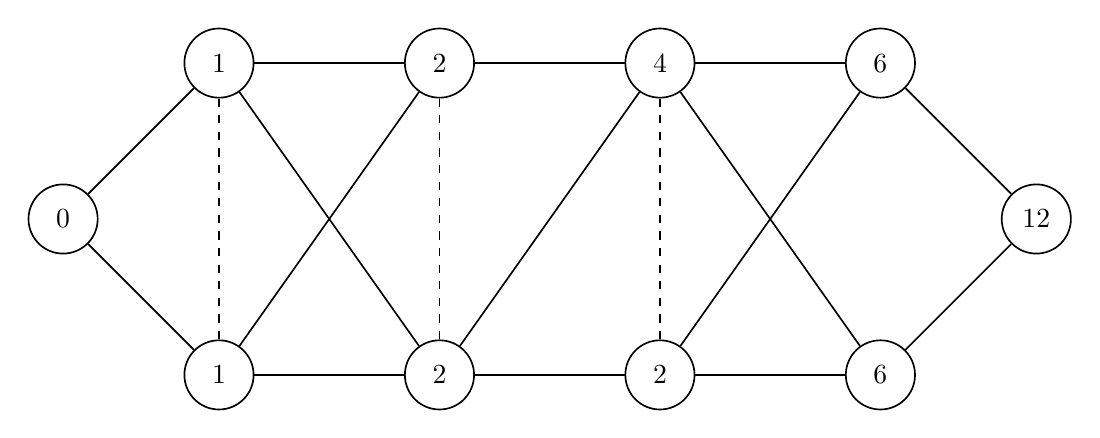
\begin{tikzpicture}[-,auto,node distance=2.8cm,semithick]
   \tikzstyle{every state}=[draw,text=black]

   \node[state] (A)                    {$0$};
   \node[state] (B) [above right of=A] {$1$};
   \node[state] (C) [below right of=A] {$1$};
   \node[state] (D) [right of=B]       {$2$};
   \node[state] (E) [right of=C]       {$2$};
   \node[state] (F) [right of=D]       {$4$};
   \node[state] (G) [right of=E]       {$2$};
   \node[state] (H) [right of=F]       {$6$};
   \node[state] (I) [right of=G]       {$6$};
   \node[state] (J) [below right of=H] {$12$};
   
   \path[dashed]
         (B) edge node {} (C)
         (D) edge node {} (E)
         (F) edge node {} (G);
   
   \path (A) edge node {} (B)
             edge node {} (C)
         (B) edge node {} (D)
             edge node {} (E)
         (C) edge node {} (D)
             edge node {} (E)
         (D) edge node {} (F)
         (E) edge node {} (F)
             edge node {} (G)
         (F) edge node {} (H)
             edge node {} (I)
         (G) edge node {} (H)
             edge node {} (I)
         (H) edge node {} (J)
         (I) edge node {} (J);
 \end{tikzpicture}
\\

\item \emph{Define a random graph $G = (n,p)$ on the set of $n$ vertices as follows: for each pair of vertices $u, v$, $\{u, v\}$ is declare to be an edge with probability $p$ independently of all the others. What is the expected number of cycles $C_4$ in this graph? For the purpose of this exercise, assume that two cycles that are obtained from each other by rotations and reflections are considered the same, but they need not necessarily be induced (ie. may contain diagonals.)} \\
\\
Looking for $E(C_4)$, by linearity of expectation we can split this problem into the sum of expectations of Bernoulli variables, with one Bernoulli variable for each possible cycle, taking the value 1 if it does appear in the graph and 0 if it does not. So, if $m$ is the total number of possible cycles,
\begin{align*}
E(C_4) = E(X_1 + \dots + X_m) = E(X_1) + \dots + E(X_m)
\end{align*}
For any given four vertices $(v_1,v_2,v_3,v_4)$ in $G$, there are three distinct cycles: $(v_1,v_2),(v_2,v_3),(v_3,v_4),(v_4,v_1)$ in edges of $G$, $(v_1,v_2),(v_2,v_4),(v_3,v_4),(v_1,v_3)$ in edges of $G$, or $(v_1,v_4),(v_2,v_4),(v_2,v_3),(v_1,v_3)$ in edges of $G$. (These are an hourglass, a bowtie, and a box.) There are $\binom{n}{4}$ ways to choose four vertices, so the total number of possible distinct cycles in $G$ is
\begin{align*}
\binom{n}{4} \cdot 3 = \frac{n! \cdot 3}{(n-4)! \cdot 4!}
\end{align*}
Because the probability that each edge will occur is independent from all others, the probability that any given cycle from the set of possible cycles will occur is simply $p \cdot p \cdot p \cdot p = p^4$, since we are only concerned with the probability that four particular edges occur. Finally, because each $X_i$ is a bernoulli variable and the $E(Y) = \sum_{r \in Y(S)} p(Y = r)r$, because all $r \in {0,1}$, we know that $E(X_i) = p(X_i)$. So
\begin{align*}
E(X_i) = p(X_i) = p^4 \\
E(C_4) = \Sigma_{all\;i}\; E(X_i) = \frac{n! \cdot p^4 \cdot 3}{(n-4)! \cdot 4!} \\
\end{align*}



\item \emph{Prove that a connected graph with $n$ vertices has exactly $n$ edges if and only if it contains precisely one simple cycle.} \\
\\
For a connected graph $G$ with $n$ vertices, \\
let $A$ mean $G$ has $n$ edges \\
let $B$ mean $G$ contains precisely one simple cycle. \\
\\
Lemma: Given a connected graph $A$ containing a simple cycle, removing an edge from within the cycle still results in a connected graph. \\
\\
Proof of lemma: \\
Let a simple cycle within $A$ consist of the vertex sequence $v_1,v_2,\dots,v_n$, where $v_n$ connects back to $v_1$. For any two vertices in the $G$, $v$ and $w$ which are connected, if we remove some edge within the cycle $(v_i,v_{i+1})$ to obtain a new graph $G'$, we can show that $v$ and $W$ are still connected in $G'$. Case one: the original path between $v$ and $W$ does not contain $(v_i,v_{i+1})$. In this case, $v$ and $w$ must still be connected since removing that edge does not effect the path. Case two: the path between $v$ and $W$ \emph{does} contain $(v_i,v_{i+1})$. In this case, we can still find a path between $v_i$ and $v_{i+1}$, by 'going around', taking the path $v_i, v_{i-1}, \dots, v_1, v_n, v_{n-1} \dots v_{i+1}$. Thus, in $G'$, we can replace $(v_i,v_{i+1})$ in the path connecting $v$ to $w$ with that vertex sequence, so $v$ and $w$ are still connected. So $G'$ is still a connected graph. \\
\\
Now, on to the original proof. \\
\\
Proof $A\to B$: \\
Let $G$ have exactly $n$ edges. By way of contradiction, assume that $G$ is acyclic. Since $G$ is connected and acyclic, by the properties of trees, it is a tree. However, trees must also have $n-1$ edges. By $A$, we know that $G$ has $n$ edges, so by contradiction, $G$ cannot be acyclic. Equivalently, it must contain at least one simple cycle. \\
\\
By way of contradiction, assume that $G$ contains two simple cycles. If so, there must be at least one edge some $(u,v)$ in cycle 1 that is not in cycle 2. Since that edge is part of a cycle, we can remove it without disconnecting the graph (by the lemma proved above). The resulting graph, which still contains cycle 2, is still connected and has $n-1$ edges. By the properties of trees, this graph is a tree. However, trees are acyclic, so we have a contradiction because our graph should still contain cycle 2. By contradiction and our reasoning above, $G$ must contain precisely one simple cycle. \\
\\
Proof $B\to A$: \\
Let our connected graph $G$ of $n$ vertices have exactly one simple cycle. We can remove a single edge from this simple cycle to obtain a new graph $G'$. \\
\\
Because $G$ is a connected graph and the we removed an edge from within a cycle, $G'$ must also be a connected graph (by the lemma proved above). Since we have removed an edge from it, $G'$ no longer contains a simple cycle. Since it contains no simple cycles, it must be acyclic. By the properties of trees, because $G'$ is acyclic and connected, it is a tree and thus must have $n-1$ edges. By construction, $G'$ has one less edge than our original $G$, so $G$ must have exactly $n$ edges.



\end{enumerate}
\end{document}
